%  OS Review 
%  LaTex version of RH's thesis - in process of being reworked
%  into a review paper.
%  With permission, used EC's naris paper tex file as a template. 
%  RH

\documentclass[11pt]{article}

% packages
\usepackage{natbib}
\usepackage{graphicx}
\usepackage[nolists]{endfloat}
\usepackage{times}
\usepackage{ifthen}
\usepackage{parskip}
\usepackage[font=sf,labelfont=bf]{caption}
\usepackage{xspace}
\usepackage[pdftex]{color}
\usepackage{pdfcolmk}
\usepackage{amsmath}
\usepackage{fixltx2e} % for \textsubscript


% line numbers
\usepackage[left]{lineno}

% variable margins
\usepackage[left=2.5cm,top=2.5cm,bottom=3.5cm,right=2.5cm]{geometry}

% this helps figure placement
\renewcommand{\textfraction}{0.0}
\renewcommand{\topfraction}{1}
\renewcommand{\bottomfraction}{1}

% spacing
\setlength{\parindent}{0in} 
\setlength{\parskip}{2\baselineskip}
\linespread{2}
\renewcommand{\baselinestretch}{1.66}\normalsize

% definitions
\newcommand{\bsf}[1]{\textbf{#1}}
\newcommand{\sem}{S.E.M.\@\xspace}
\newcommand{\degree}{$^o$\@\xspace}
\makeatletter
\setlength{\@fptop}{0pt}
\makeatother
\newcommand\given[1][]{\:#1\vert\:} % found this on stackexchange

% bib
\bibliographystyle{apa}
\let\cite=\citep
\let\citeN=\citet
\let\citeNP=\citealt
\renewcommand{\bibfont}{\footnotesize}
\setlength{\bibsep}{2pt}

\begin{document}

{\Large\bf Fancy title goes here}

%{\bf Authors}: James E.\ Carmichael\textsuperscript{1}, Jimmie
%M.\ Gmaz\textsuperscript{1}, Matthijs A.\ A.\ van der
%Meer\textsuperscript{1*}

{\bf Authors}: To be filled out...

\textsuperscript{1}Department of Psychological and Brain Sciences,
Dartmouth College, Hanover NH
03755\\ %\textsuperscript{2}Department of Biology and
%\textsuperscript{3}Centre for Theoretical Neuroscience, University of
%Waterloo, Canada\\

\textsuperscript{*}Correspondence should be addressed to MvdM,
Department of Psychological and Brain Sciences, Dartmouth College, 3
Maynard St, Hanover, NH 03755. E-mail: {\sffamily mvdm@dartmouth.edu}.

\textbf{Number of Figures:} x\\
\textbf{Number of Tables:} x\\
\textbf{Total Word Count:} x\\
\textbf{Abstract Word Count:} x\\
\textbf{Introduction Word Count:} x\\
\textbf{Discussion Word Count:} x\\

\textbf{Acknowledgments}: To be filled out...

\textbf{Conflict of Interest}: The authors declare no competing
financial interests.\\

\newpage
\linenumbers

\section*{Abstract}
% This is to help lay out sections of the paper...
% Review will ultimately need a completely new abstract... 

Behavior is constantly modulated by ever-changing constellations of cues
that determine the behaviorally relevant state. For example, a vehicle
approaching the crosswalk signals a shifted state in which it is no longer
appropriate to cross the road. To date, very little is known about the neural
substrates underlying state shifts. This is surprising given how important 
state identification is to exhibiting contextually appropriate behavior. First, 
we review the existing literature, and point to models that provide an 
especially useful conceptual framework for dealing with this problem. Second, 
we report the results of three experiments in which we set out to model state 
shifts in rats by employing two related tasks: serial biconditional 
discrimination (BD), and negative occasion setting (NOS) (both Pavlovian, and 
involving discrete cues). In order to successfully predict trial reinforcement 
value in the former task, animals had to be sensitive to the following cue 
combinations: V1 $\rightarrow$ A1 $+$, V2 $\rightarrow$ A1 $-$, V1 $\rightarrow
$ A2 $-$, and V2 $\rightarrow$ A2 $+$, where `$+$' denotes reward, and `$-$' 
denotes no reward. We hypothesized a state shift in representing A1 (and A2) 
depending on the identity of the cue preceding it. In Experiment 1, trials were 
presented in pseudorandomized order, and in Experiment 2, trial ordering was 
blocked. Strikingly, neither experiment promoted successful acquisition of 
biconditional discrimination. As such, we shifted to a NOS task 
\cite{Holland1999} that included a conditional discrimination between L $
\rightarrow$ T $-$ and T $+$ trials. Surprisingly, this established design was 
also not learned by the group. The implications of these findings are 
discussed. At the outset, we intended to carry out in-vivo electrophysiological 
recordings from CA1 while rats performed the task in order to characterize 
ensemble firing of putative state shifts.

\section*{Significance Statement}

Significance statement will eventually go here...

\newpage

\section*{Introduction}

The environment is replete with ambiguous events whose meaning requires moment-
to-moment disambiguation. This presents a high-stakes challenge to behaving 
organisms, given that deciphering an event's current meaning often makes the 
difference between life and death. In the literature, this general problem has 
been illustrated through various examples. For example, a crosswalk is 
generally thought of as a safety cue signaling where the road can be traversed. 
However, we still look left and right before crossing, because we understand 
that the crosswalk's safety signaling property is cancelled when there is a car 
bolting towards it \cite{Meyer2016}. Another related example concerns the 
multiple meanings of individual words - for instance, when ``Fire!'' is cried 
out in the shooting gallery, it holds a meaning that is very different from 
when it is cried out in a bank \cite{Bouton1994}. Each of these anecdotal 
examples involves an ambiguous event that needs to be resolved by paying 
attention to other relevant factors. Crucially, the examples differ in terms of 
what these factors are; in the former case, a discrete stimulus mediates the 
resolution (i.e., a moving car), while in the latter case, a complex stimulus 
configuration fulfills this role (i.e., a physical context such as the interior 
of a bank). Note, the notion of context is one that is highly relevant to the 
discussion of ambiguity resolution; in order to emit the appropriate response 
when confronted with an ambiguous stimulus, the agent must first identify the 
current context, or state. Framed in these terms, context simply acts as a 
disambiguator. There is an extensive literature discussing the various roles of 
context, but a detailed treatment of the topic is beyond the scope of this 
review (see \citeNP{Bouton1994,Bouton2004,OKeefe1978,Nadel1980,Rudy2009}). For 
sake of consistency, we will refer to the disambiguating factor as the 
``feature'', and to the ambiguous event as the ``target'' \cite{Bouton2007}. 
Overall, it is clear that situations involving ambiguity resolution pose a 
nontrivial problem - the brain needs to identify the relevant feature, and use 
it to represent a neural difference across otherwise perceptually identical 
instances of the target. 

In this article, we review tasks that involve ambiguity resolution with special 
emphasis on occasion setting (see Figure 1a). First, we describe the 
computational problem underlying ambiguity resolution as it is embodied in OS, 
and discuss four identifying features that make OS distinct from related 
behaviors. We go on to review existing accounts of OS and point to some of 
their pitfalls - we argue that each account lacks the generality to explain all 
domains of ambiguity resolution, and that neither captures all four features of 
OS. For this reason, we propose an alternative account - one that relies on the 
inference of latent causes and the assignment of state-dependent action values 
\cite{Gershman2012}. We give an example of such an account, and briefly 
describe how it deals with OS. Lastly, we demonstrate the account's utility by 
pointing to its behavioral and neural predictions. 

\begin{figure}[h]
\centering
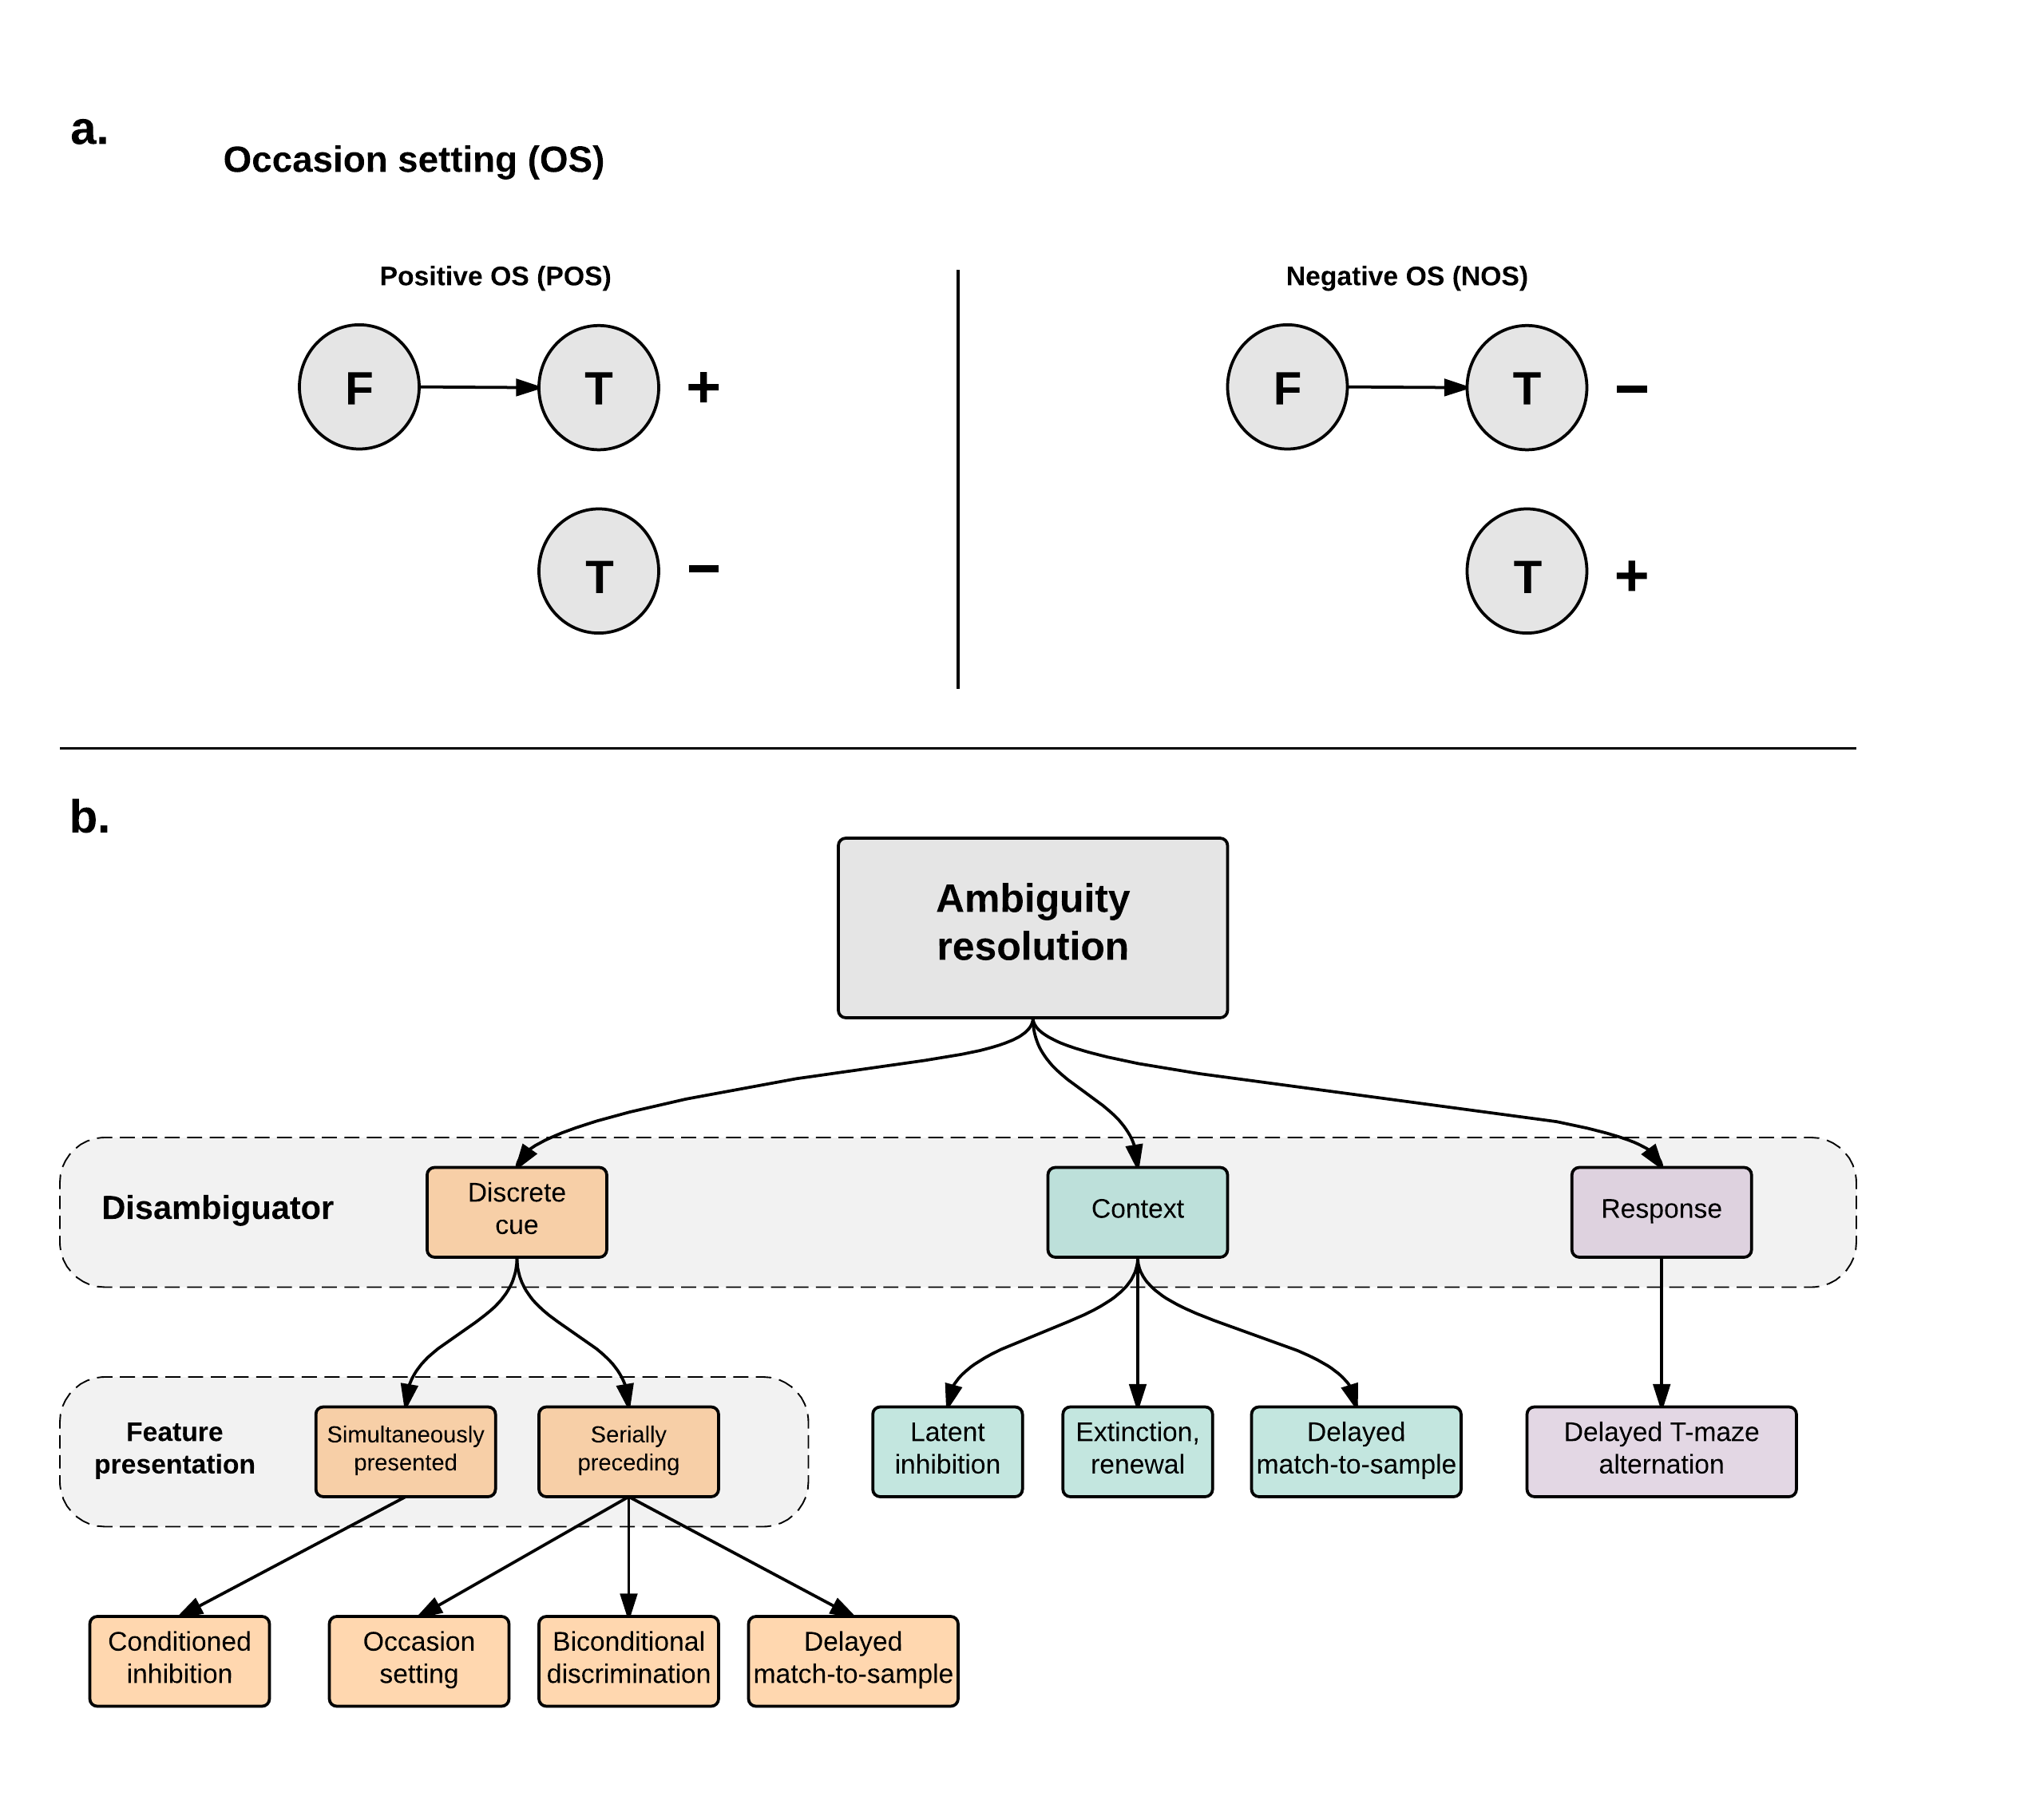
\includegraphics[width=\textwidth]{Figures/Fig1}
\caption{\bsf{(a)} Positive occasion setting (left) and negative occasion setting (right). ``F'' denotes the feature cue, ``T'' is the target, and ``$+$'' is reward (``$-$'' is its omission). \bsf{(b)} Tree diagram describing relationships between tasks involving ambiguity resolution. Tasks are separated into three categories depending on whether the feature is discrete, contextual, or a response. Within the discrete-feature category, tasks are further categorized by whether the feature serially precedes the target or is presented with it simultaneously.}
\label{fig:ambiguityTasks}
\end{figure}

\section*{Occasion setting and ambiguity resolution}

In OS, subjects learn to identify the meaning of a target cue (T) depending on 
whether a feature cue (F) precedes it or not. Tasks that involve OS therefore 
consist of two trial types: one in which the target is presented alone (T 
trials), and one in which the target is serially preceded by the feature (F $
\rightarrow$ T trials). Framed in these terms, it is clear that OS involves 
ambiguity resolution, since the meaning of T requires trial-by-trial 
disambiguation - to this end, animals must learn to use the presence or absence 
of F as a signal to inform the present meaning of T.

In positive occasion setting (POS), F $\rightarrow$ T trials result in reward, 
while T trials result in no reward - in this case, the feature is referred to 
as a positive occasion setter, since it ``sets the occasion'' for the target's 
reward prediction value. Conversely, in negative occasion setting (NOS), F $
\rightarrow$ T trials result in no reward, while T trials result in reward - 
here, the feature is referred to as a negative occasion setter, as it cancels 
the target's reward prediction value. The arrow symbol (``$\rightarrow$'') 
between F and T represents the fact that OS paradigms typically include a 
temporal gap (i.e., an inter-stimulus interval, or ISI) between the feature and 
the target - indeed, the presence of the ISI has proven to be a crucial factor 
for promoting the acquisition of OS as opposed to other forms of learning - 
e.g., conditioned inhibition \cite{Rescorla1969} - that are learned when F 
offset and T onset are temporally contiguous, or when F and T are presented 
simultaneously \cite{Holland1992}. 

Overall, OS has received a great deal of attention from learning theorists, as 
occasion setters hold properties that make them distinct from regular 
conditioned stimuli (CSs). First, it has been demonstrated that a CS with 
positive reward predictive value (i.e., an exciter) often comes to elicit a CS-
specific conditioned response. In rats, for instance, auditory exciters elicit 
head jerking, while visual exciters elicit rearing \cite{Holland1984}. In OS, 
the feature is only used in order to inform the current value of the target; 
thus, any conditioned responding is specific to the modality of the target, not 
the feature. For example, when a light feature is trained with a tone target in 
a POS paradigm, the resulting CR on reinforced trials would be that elicited by 
the tone \cite{Ross1981}. Furthermore, occasion setters are immune to 
counterconditioning. For instance, when a negative occasion setter is 
repeatedly paired with reward, its capacity to act as a negative occasion 
setter goes largely unaffected \cite{Holland1991, Holland1992}. Additionally, 
an occasion setter's properties are specific to its target, and do not transfer 
well to cues that have not been trained as targets of other occasion setters 
(i.e., non-target cues). Lastly, there is a remarkable difference between NOS 
and POS that stems from the amount of training required until a robust 
discrimination has been acquired - it turns out that NOS is acquired 
significantly slower than POS (see Figure 2). This has often been referred to 
as the feature-positive effect \cite{Jenkins1970}, and has typically been 
observed in behavioral paradigms involving a simultaneous presentation of the 
feature and the target (i.e., a FT compound). More specifically, animal 
\cite{Gonzalez2003} and human \cite{Wheeler2006} studies found that when the FT 
compound is first paired with reward, and then T is presented individually in 
extinction, the decrement in responding to T is significantly greater than when 
the reverse scenario takes place - i.e., when T is first reinforced, and then 
tested as compound FT. The feature-positive effect has often been described as 
an asymmetry in stimulus generalization between discrete cues and compounds 
\cite{Bouton2012}. It is plausible that in the case of OS, the feature-positive 
effect is explicable in similar terms. In any case, any realistic account of OS 
must be able to make sense out of this phenomenon, as it likely reflects an 
important difference in the neural processes that govern the acquisition of POS 
as opposed to NOS. In summary, we propose the following four criteria as a 
loose benchmark (see below) for a successful model of OS:

\begin{enumerate}
   \item[(1)] Response form is target-specific.
   \item[(2)] Occasion setters are immune to counterconditioning.
   \item[(3)] The properties of an occasion setter do not transfer well to a 
   non-target cue.
   \item[(4)] NOS is acquired significantly slower than POS (feature-positive 
   effect).
\end{enumerate}

\begin{figure}[h]
\centering
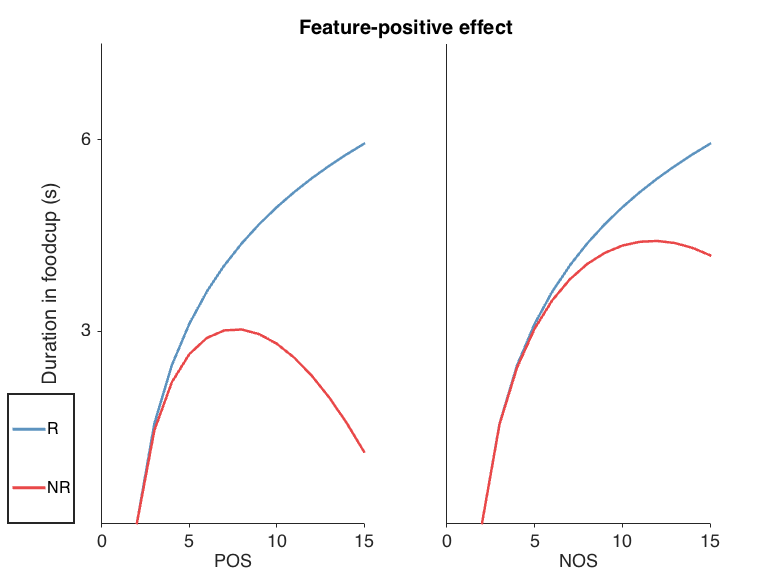
\includegraphics[width=\textwidth]{Figures/Fig2}
\caption{Feature-positive effect. R denotes the rewarded trial type, and NR the 
unrewarded trial type. The simulated acquisition curves demonstrate the feature-
positive effect, as in the case of POS, discrimination between R and NR trials 
occurs earlier than in NOS. The diagram is based on data in \citeN{Holland1999}, 
and \citeN{Bouton2011}.}
\label{fig:FPeffect}
\end{figure}

% Paragraph to caution reader against viewing our benchmarks as dogma
It is necessary to point out that not all of the above ``benchmarks'' have been 
equally well established. In one study, rats trained in an OS paradigm passed 
the requirement for response form (1), but not for counterconditioning (2) 
\cite{Moreira2003}. The data on OS transfer effects (3) have been particularly 
variable - for instance, occasion setting properties do transfer (albeit not 
completely) to a non-target cue if it is similar to the original target 
\cite{Swartzentruber1995}, or if both cues predict the same reinforcer (i.e., 
US-specific transfer; see \citeNP{Bonardi2012,Bonardi2017}). Indeed, the 
feature-positive effect (4) seems to be among the most consistent results, 
making appearance in a large variety of behavioral tasks (see 
\citeNP{Jenkins1970,Bouton2011,Bouton2012,Holland1999}). In our view, these 
inconsistencies further underscore the need for novel theoretical 
frameworks in OS. 

A large number of behavioral tasks apart from OS have modeled ambiguity 
resolution. Figure 1b displays the tasks as categorized by identity of the 
feature (e.g., discrete cue, context, response), and by whether the feature 
serially precedes or co-occurs with the target. It is interesting to note that 
some of the tasks were not originally designed to tackle ambiguity resolution. 
For example, the delayed match-to-sample design was employed to study working 
memory \cite{Miller1996}. This said, the task clearly involves trial-by-trial 
ambiguity - the design involves instances of a target cue whose immediate 
meaning depends on whether a previously presented feature is identical to it or 
not. Overall, it is useful to have an explicit statement of the computational 
problem the brain must tackle in order to resolve ambiguities successfully. To 
this end, the OS literature is especially informative, as it involves models 
that deal with this general problem. Indeed, OS holds a somewhat unique 
position in the task hierarchy depicted in Figure 1b. First, it is arguably the 
simplest instance of ambiguity resolution, as both the target and the feature 
are discrete cues, as opposed to more complex stimulus configurations. 
Moreover, the discreteness of the feature implies that it can be presented at 
will, which grants the experimenter unique control over the current meaning of 
the target. This aspect is particularly useful for studying the neural 
substrates underlying the different meanings of the target across rewarded and 
unrewarded OS trial types.

\section*{Existing accounts of OS}

The unique properties of occasion setters have made them a challenge to 
standard models of associative learning, such as the Rescorla-Wagner model 
\cite{Rescorla1972}. The model developed by Rescorla and Wagner details the 
process by which environmental stimuli come to predict the occurrence (or non-
occurrence) of behaviorally salient events (e.g., reward, footshock). These 
events are thought to support a threshold of conditioning ($\lambda$) that 
reflects their surprisingness. When confronted with such an event, the model 
assumes that all neutral cues (e.g., lights, tones, etc.) present at the time 
of the event come to accrue `associative strength' (parameter V in the model) 
that decrements the surprisingness of the event - in other words, the neutral 
cues become predictive of the upcoming event by virtue of their non-zero V. For 
each cue, the change in associative strength occurs on a trial-by-trial basis, 
and is proportional to the difference between the surprisingness of the event, 
and the sum of the associative strengths of all cues present ($\lambda - \sum
$V). Given that the Rescorla-Wagner model does not include temporal dynamics, 
it has no way of using the discontiguous occasion setter to acquire a 
discrimination between F $\rightarrow$ T and T trials. As such, the model 
predicts that F remains a neutral cue, while each rewarded T accrues positive 
V, and each unrewarded T accrues negative V. In this case, the discrimination 
is never achieved. Another possibility is to assume stimulus contiguity on F $
\rightarrow$ T trials. In this case, the model solves the task by accruing 
positive V to F in POS, and negative V to F in NOS. However, since this 
discrimination relies on direct associations between F and the outcome, it 
fails both the counterconditioning (2) and transfer requirements (3).
	
This challenge has precipitated the development of novel accounts aiming to 
explain the properties of occasion setters, as well as reconcile them with 
associative accounts of classical conditioning. In this section, we discuss 3 
existing accounts of OS: hierarchical theory, configural theory, and the SLH 
model (Figures 3 and 4). We give a brief description of each, and discuss 
specific predictions pertaining to the 4 criteria we identified. 

\begin{figure}[h]
\centering
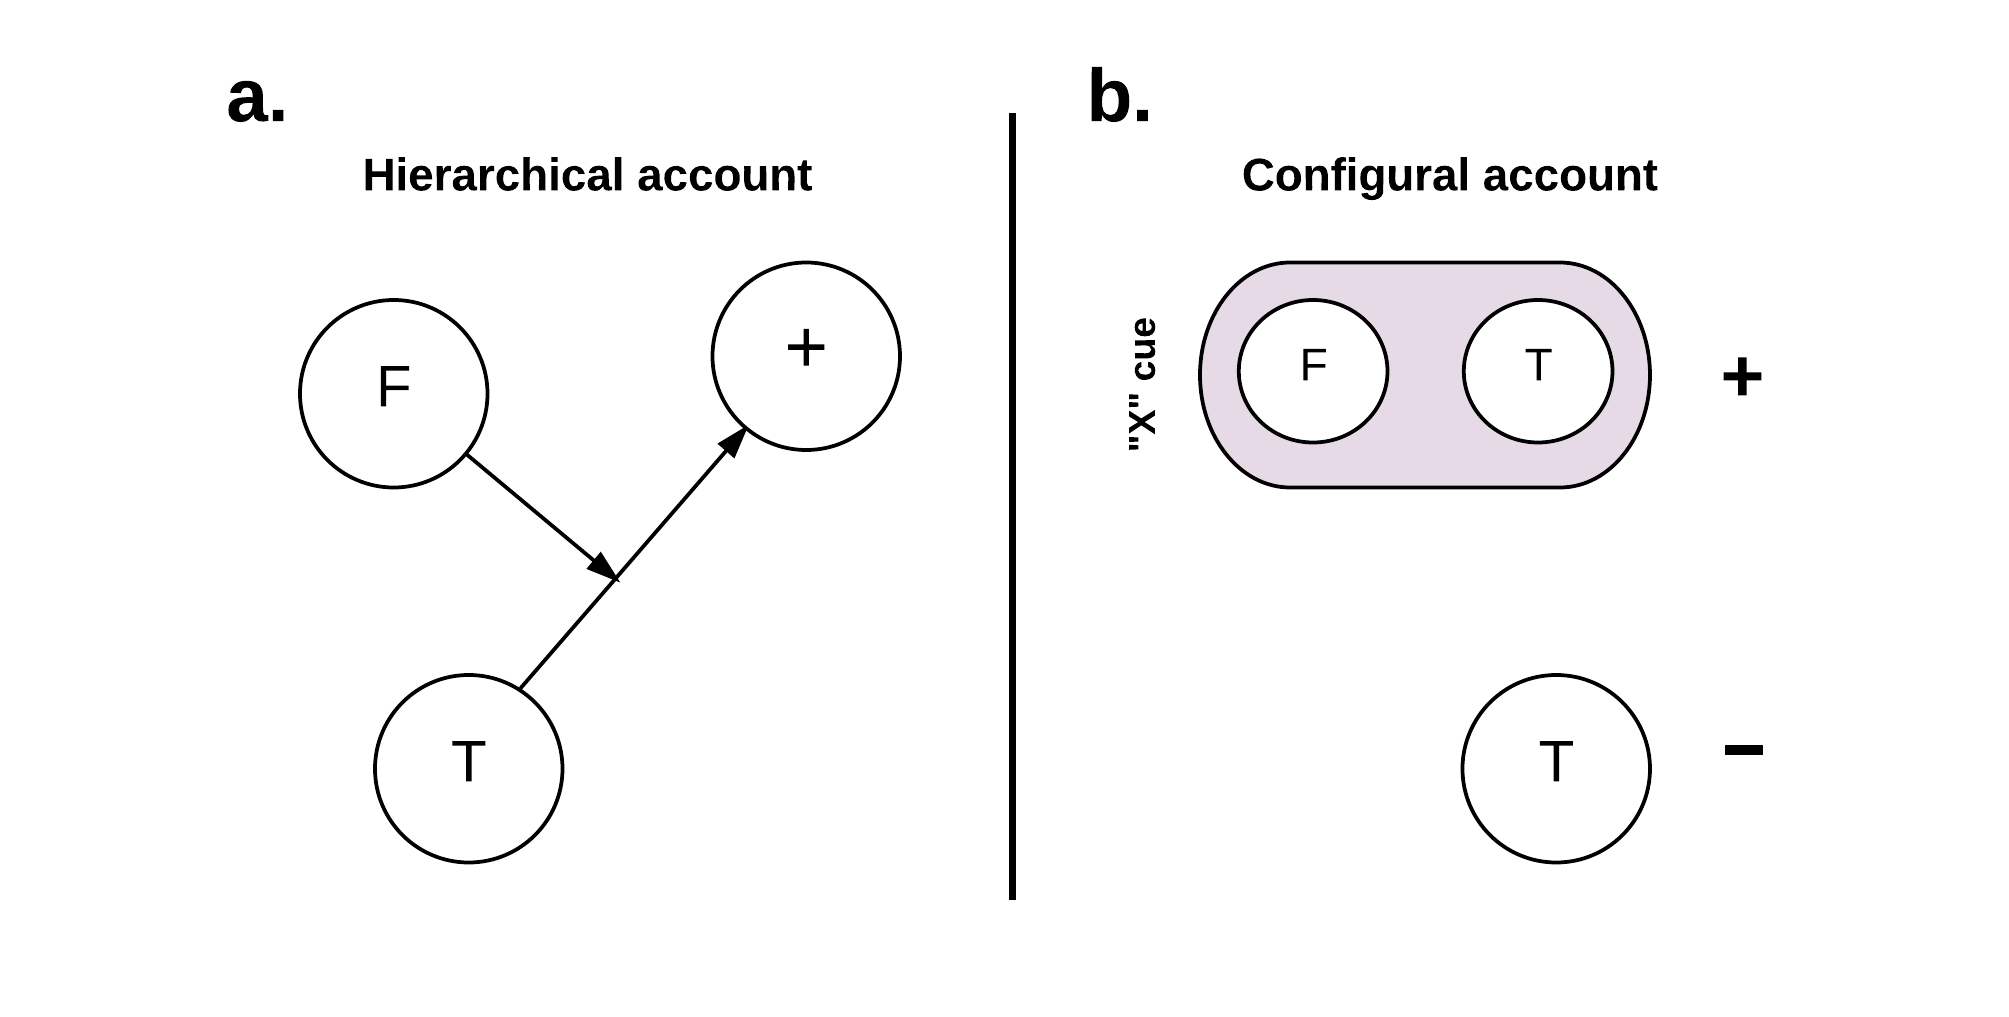
\includegraphics[width=\textwidth]{Figures/Fig3}
\caption{Two accounts of OS. \bsf{(a)} The hierarchical account of OS posits 
that the feature (F) gates the target's (T) association with reward ($+$). 
\bsf{(b)} The configural account assumes that all cues present on a given trial 
are encoded as a configural stimulus comprising of cue-specific and configure-
specific components; for example, on an F $\rightarrow$ T$+$ trial, cues are 
represented as a configure X consisting of F-specific, and T-specific 
components.}
\label{fig:traditionalAccounts}
\end{figure}

{\bf Hierarchical theory}. This account claims that the occasion setter comes 
to modulate the specific association between the target and reward (Figure 3a). 
A specific instance of this idea is given by \citeN{Bouton1998}; in NOS, for 
example, the target is thought to develop a simple excitatory association with 
reward on T$+$ trials. On F $\rightarrow$ T$-$ trials, however, the target 
forms an inhibitory association with reward, such that this association is only 
active in the presence of the feature. In this manner, the feature comes to 
hierarchically gate the active association between the target and reward 
\cite{Bouton1998}. Assuming that the nature of conditioned responding is given 
by the identity of the response-eliciting CS, hierarchical theory is consistent 
with the response form requirement (1). Moreover, the specificity of F's 
modulatory influence is consistent with immunity to counterconditioning (2) and 
transfer effects (3); In the case of counterconditioning, it has been argued 
that altering the feature's associative relationship with the reinforcer does 
not change its relationship with the target-US associative link (`US' denotes 
unconditioned stimulus, which is reward in this case). Interestingly, 
hierarchical theory can even account for US-specific transfer - one of the more 
nuanced OS phenomena - which is explained as a generalization effect that stems 
from the similarity of associations involving the same reinforcer; more 
specifically, if F acts on a T-US$_{1}$ associative link (where T was trained 
as a target of F), then the occasion setting properties of F will likely 
generalize to a C-US$_{1}$ link, even though C was never trained as a target of 
F - this is due to a similarity between the T-US$_{1}$ and C-US$_{1}$ 
associations by virtue of their shared reinforcer.

{\bf Configural theory}. In contrast to the hierarchical account stands 
configural theory, which states that on F $\rightarrow$ T trials, the feature 
and the target are encoded together as a unique configural stimulus X 
\cite{Pearce1987,Pearce1994}. Under this assumption, OS is reduced to a simple 
discrimination between X and T trials, where X is distinct from its component 
elements F and T. From this, it follows that counterconditioning F would do 
little to change responding to X. Similarly, preceding a non-target cue with F 
would simply create a new configure X', a stimulus entirely distinct from X. So 
far, configural theory is consistent with immunity to counterconditioning (2), 
and transfer effects (3). Furthermore, some have claimed that since the 
presentation of F precedes T in time, the configure X is actually formed by 
encoding the trace of F together with T \cite{Holland1992}. This would make X 
more similar to T by virtue of stimulus generalization, and responding to X 
should therefore bare resemblance to a response to T. As such, configural 
theory is also consistent with the response-form requirement (1). However, 
without making ad-hoc adjustments to the theory, there is no reason why NOS (X
$-$ and T$+$ trials) should be acquired slower than POS (X$+$ and T$-$ trials) 
- as such, the account cannot explain the feature-positive effect (4). 
Interestingly, there is a variant of configural theory, which explains the 
feature-positive effect by positing that the F $\rightarrow$ T configure is 
composed of feature-specific elements, target-specific elements, and elements X 
that are unique to the configure \cite{Rescorla1973}. In the case 
of POS, positive V would be split equally among elements of the F $\rightarrow$ 
T configure (F, T, and X). As such, the small positive V accrued to T would be 
quickly counteracted on T$-$ trials. In contrast, in NOS, the large positive V 
accrued to T would take more time to counteract on F $\rightarrow$ T trials, 
thereby delaying acquisition of the discrimination. Note that this configural 
assumption makes OS tractable for elemental theories such as the Rescorla-
Wagner model. Indeed, this is a large reason for the account's shortcomings - 
for example, by accruing V to F during OS acquisition, F becomes sensitive to 
counterconditioning. Lastly, configural theory struggles to explain some of the 
more nuanced OS-related transfer effects. For instance, it fails to explain US-
specific transfer. This is the case since the account only assumes 
generalization by virtue of cue similarity (e.g., responding to an AX configure 
might generalize to a BX configure by virtue of the shared `X' elements), but 
not by virtue of shared reinforcer identity. For this reason, hierarchical 
accounts have often been deemed to better reflect the process by which OS is 
learned \cite{Holland1992,Bonardi2017}.

{\bf SLH model}. Each of the above-discussed accounts involves a tradeoff 
between aspects that make it consistent with OS along certain dimension, but 
not along others. For example, hierarchical theory can explain 
counterconditioning and transfer effects \cite{Bonardi2017}, but not the 
feature-positive effect. On the other hand, one version of configural theory is 
in good position to explain the feature-positive effect, but not certain 
transfer effects \cite{Bonardi2017}. The unique problems associated with the 
hierarchical and configural theories of OS invite a unified model exploiting 
the advantages of each, whilst avoiding their respective pitfalls. This account 
amalgamation was achieved in the SLH connectionist model \cite{Schmajuk1998}. 
Overall, the model architecture is that of a connectionist network comprising 
layers of units that represent relevant events (e.g., features, targets, 
configures, etc.), and edges between vertices that hold associative strengths 
(Figure 4). Conditioned stimuli (contexts and discrete cues) are represented at 
the input-unit layer, while configural stimuli are represented at the hidden-
unit layer. Each input-unit forms a direct association with a corresponding 
output-unit (e.g., VS$_1$ for input unit A), as well as with every unit in the 
hidden layer (e.g., VSH$_1$ for input unit A). Hidden units also form 
associations with the output layer (e.g., VH$_1$ for hidden unit H), which 
means that each CS forms a direct association with the output layer, as well as 
an indirect one via the hidden layer. Note that each unit holds an additional 
trace memory parameter - trS for input units, and trH for hidden units - which 
reflects the activation level of the corresponding unit. In other words, when 
the unit is activated, its trace parameter value goes up, and decays over time. 
Stimulus associations are updated according to the Rescorla-Wagner rule, with 
the exception that change in associative strength is additionally weighted by 
the trace parameter: $\lambda - \text{B}$, where B $= \sum$VS$_{\text{i}}$trS
$_{\text{i}} + \sum$VH$_{\text{j}}$trH$_{\text{j}}$, the overall US expectancy. 
Crucially important is the fact that the subset of output units associated with 
a given input (e.g., VS$_1$ and VH$_1$ for input-unit A) feeds into a final 
unit that defines the conditioned response. This allows the quantification of 
CS-specific response form, a crucial asset for determining the nature of 
underlying learning upon simulation of OS.\footnote{This aspect is an extension 
to a previous version of the same model; see \citeN{Schmajuk1992}} In the 
original paper \cite{Schmajuk1998}, the authors demonstrate that SLH can 
simulate POS and NOS in a manner that is consistent with appropriate response 
form (1), counterconditioning phenomena (2), and transfer effects (3). 

\begin{figure}[h]
\centering
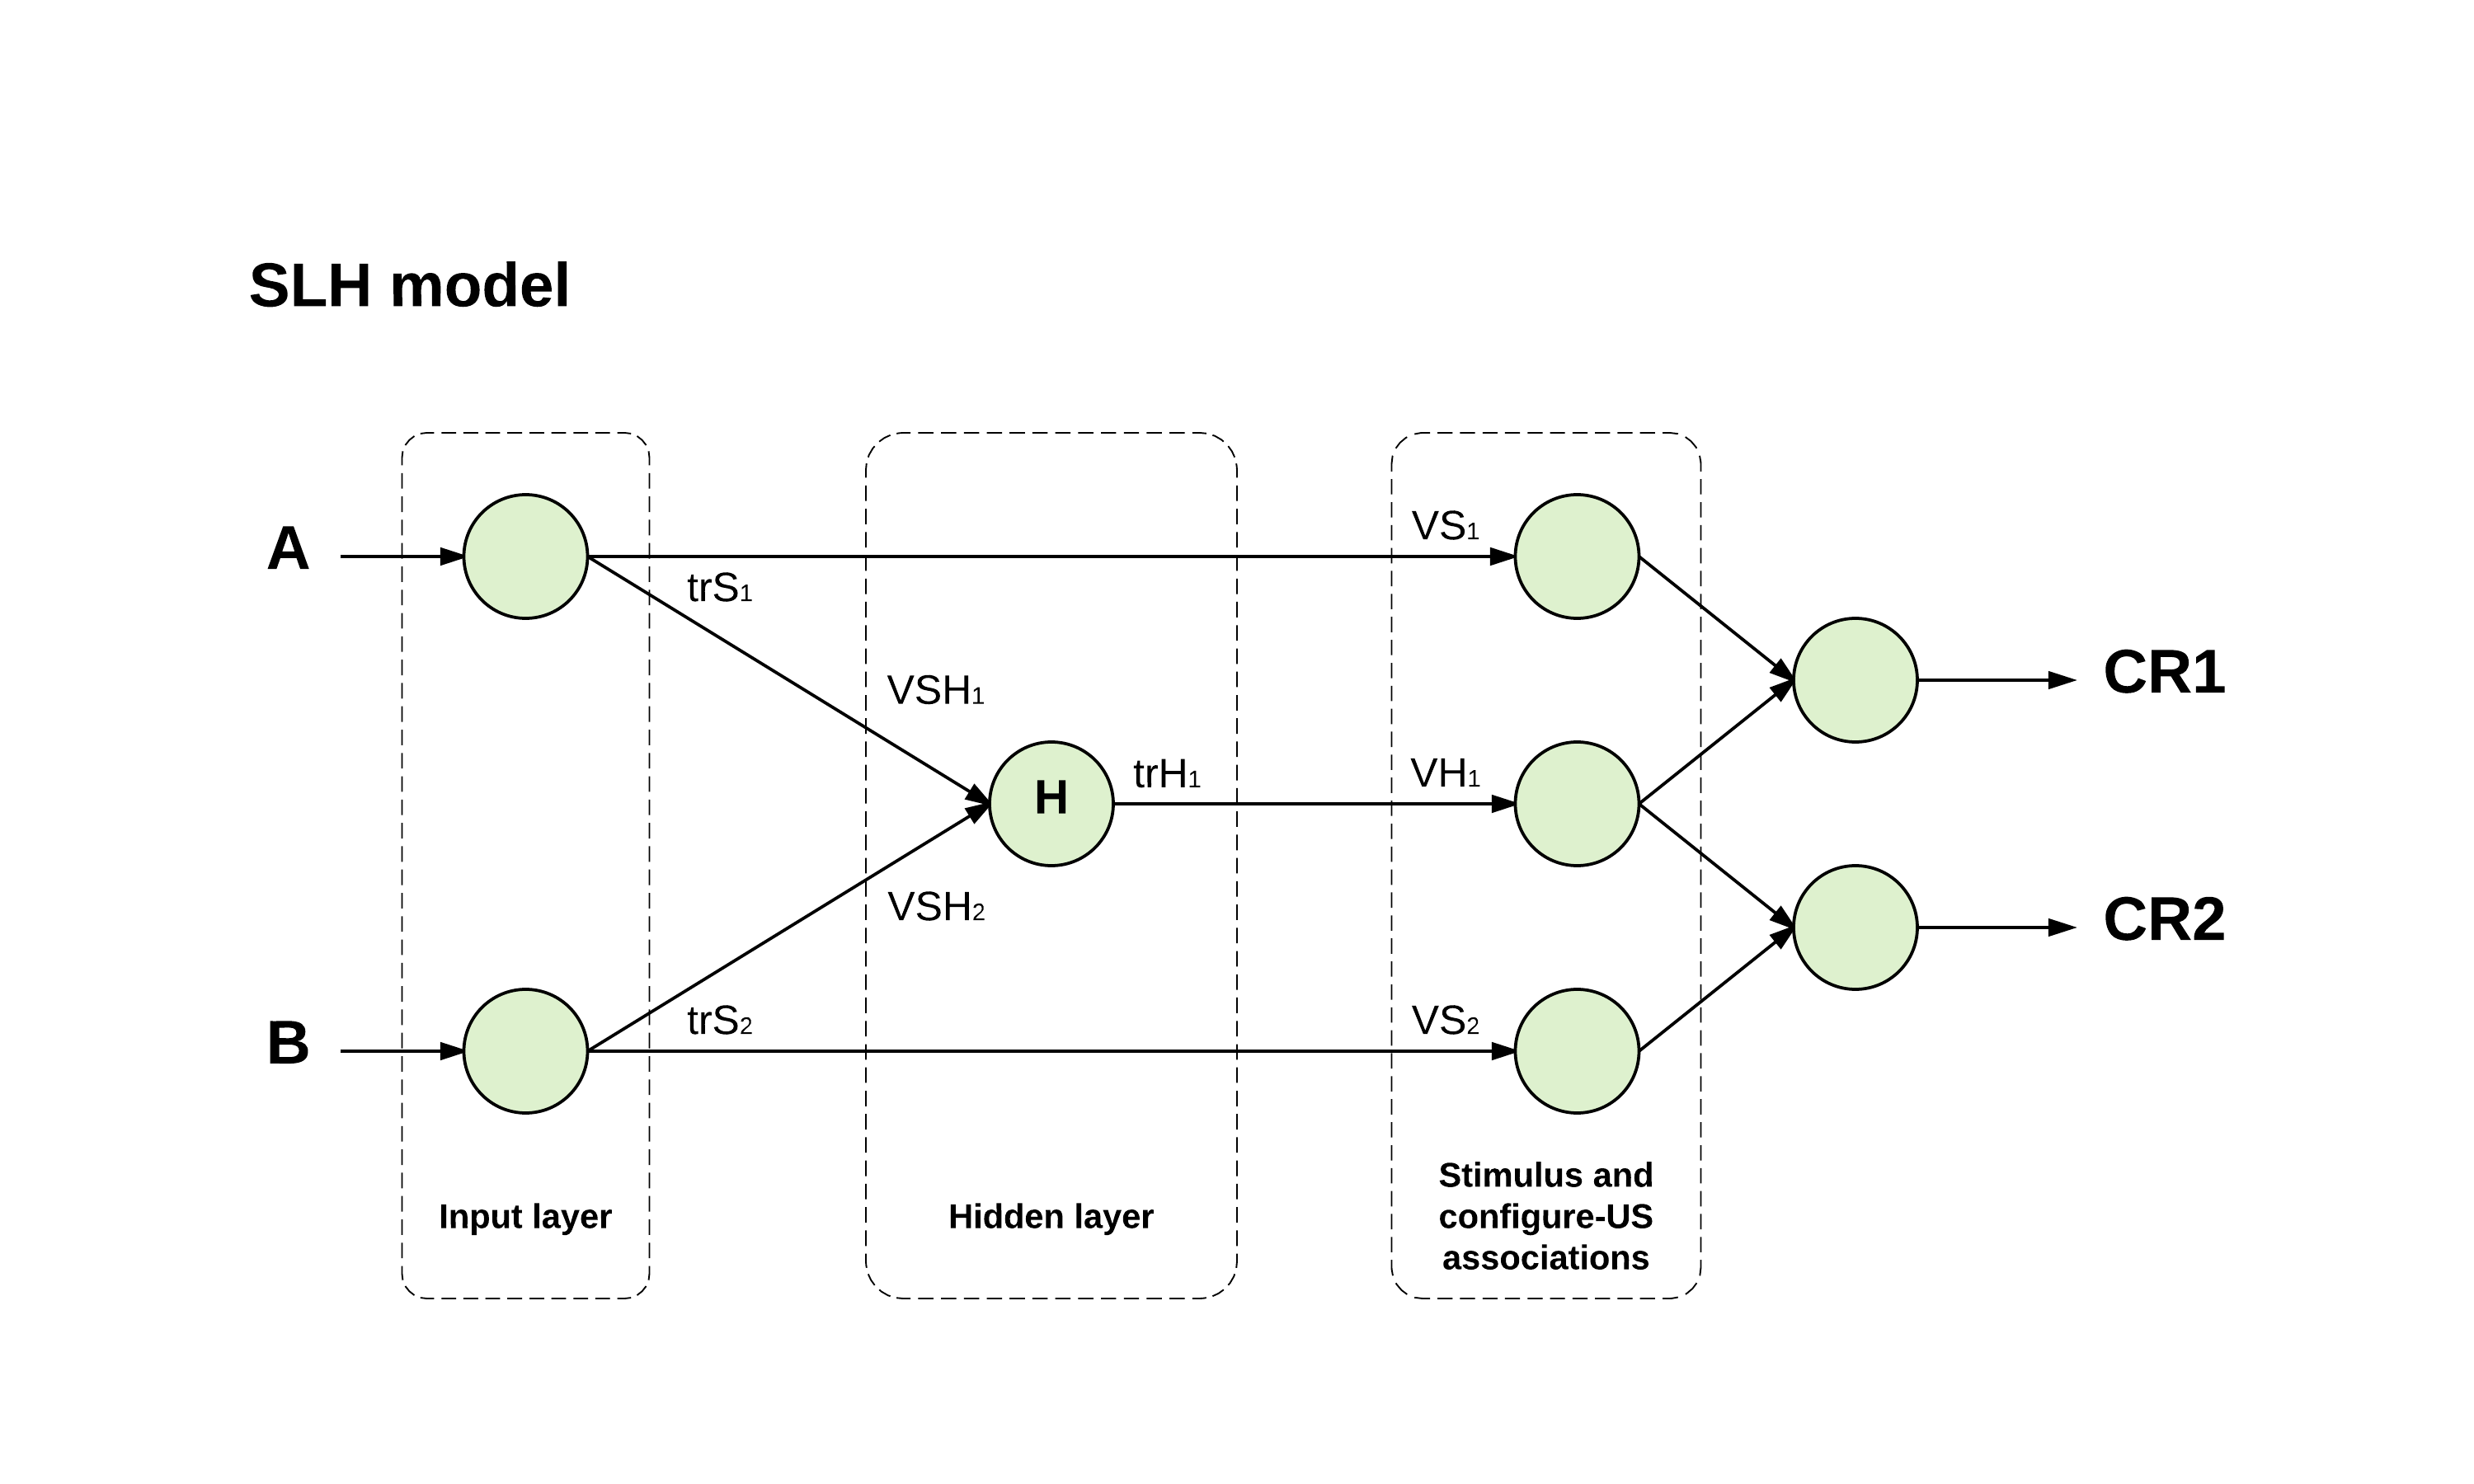
\includegraphics[width=\textwidth]{Figures/Fig4}
\caption{The SLH connectionist model comprises an input layer, a hidden layer, 
and an output layer. A, B = conditioned stimuli; trS = trace memory of a 
stimulus; H = hidden-unit representing a configuration of A and B; VSH = 
association between conditioned stimulus and hidden unit; trH = trace memory of 
a hidden unit; VS = direct association between conditioned stimulus and outcome; 
VH = direct association between hidden unit and outcome; CR = conditioned 
response.}
\label{fig:SLH}
\end{figure}

Despite these strong points, the model does not seem to account for the 
feature-positive effect; while this phenomenon is never explicitly mentioned in 
the text, the simulated acquisition curves for POS and NOS do not suggest any 
differences in acquiring the former over the latter (see Figures 15 and 18 in 
\citeNP{Schmajuk1998}). Overall, the connectionist model substitutes the 
problem of acquiring task structure for that of acquiring appropriate parameter 
weights; while this approach is effective for learning about a specific 
instance of a complex task space, it has been argued that it leads to data 
overfitting, detectable through cross-validation on a separate data set 
\cite{Fuhs2007}. This reveals a disadvantage that is common across all existing 
accounts of OS, which is a lack of generality. Indeed, neither hierarchical nor 
configural theory make it clear how to deal with instances of ambiguity 
resolution beyond the ones inherent in OS. 

In conclusion, while the SLH model meets a number of criteria that distinguish 
OS from other forms of learning, its ``learning of weights'' approach makes it 
liable to overfitting, and detracts from its potential to act as a model for 
ambiguity resolution more generally. Overall, each of the existing accounts is 
unsatisfactory, as it either does not explain all four aspects of OS, or is too 
specific to OS to be able to account for other forms of ambiguity resolution. 
For this reason, we highlight a framework that relies on partitioning the 
environment into relevant states, such that an event's meaning comes to depend 
on the state that is currently active. This general approach has brought about 
unprecedented strides in the domains of reinforcement learning 
(\citeNP{Sutton1998,Maia2009}), and has also been useful in explaining 
classical conditioning phenomena (see 
\citeNP{Courville2006,Redish2007,Fuhs2007,Gershman2010a,Gershman2010b,Gershman2012}). 
In the following sections, we argue that a state-based framework is just as 
useful in accounting for OS, and ambiguity resolution more broadly.

\section*{Towards a new theory of OS\footnote{This section introduces computational models that have yet to be fully explored as potential explanatory frameworks for OS and ambiguity resolution. Each model is explored with the intention to give the reader an intuitive understanding of how it might solve OS; however, this level of description necessarily leaves out a great deal of the mathematical and statistical underpinnings that underlie each model's inner workings; for these details, we refer the reader to the publications cited throughout the text.}}

In order to demonstrate the utility of a state-based framework, it is 
informative to consider OS through the lens of temporal difference 
reinforcement learning (TDRL) (\citeNP{Sutton1998,Maia2009,Niv2009}), a 
learning algorithm with impressive scope and generality. TDRL assumes that the 
environment can be parsed into distinct states, such that each state is 
associated with a set of possible actions and rewards. Performing a state-
related action may lead to a state transition, and associated reinforcement. 
These reinforcement values are then propagated back in time, and become 
associated with states in the past in order to signal the amount of 
reinforcement that is reachable from them. Overall, TDRL is an algorithm aimed 
at identifying sequences of state-related actions that reap the greatest 
expected reinforcement. Assuming that F $\rightarrow$ T and T trials can be 
encoded as separate states, TDRL could easily solve OS by learning that T 
signals reward in one state, but not in the other. If F merely served to toggle 
the correct state, its properties would be consistent with those of an occasion 
setter. More specifically, changing the F-outcome association would not affect 
the feature's role in state-toggling (2). The feature would only affect the 
meaning of targets whose meaning is tied to the state toggled by F (3), and 
since F only serves to establish the active state, all state-dependent 
responding would necessarily be target-specific (1). Amazingly, having states 
enter the picture provides explanatory power to account for three of the four 
key aspects of OS. Indeed, by reframing OS as a problem involving the 
acquisition of state-dependent event relations, TDRL may be exceptionally well 
positioned to explain ambiguity resolution more broadly - for example, the same 
process can be applied in order to give an algorithmic description of the 
delayed match-to-sample task. 

Despite TDRL's generality, the default model involves the significant setback 
of assuming that the state space is given. However, the major challenge of OS 
is to \textit{identify} the correct states. Once this has been achieved, 
learning the appropriate action values is a rather trivial problem. Thus, 
unless it specifies how correct states are inferred, TDRL cannot be a viable 
explanation of OS. As is becoming increasingly clear, the problem of state 
learning is highly relevant to the discussion of OS. In order to begin to 
address this problem, we review a Bayesian statistical model that has yet to be 
explored in the domains of OS and ambiguity resolution more broadly.

\citeN{Courville2006} present a generative Bayesian model that reframes 
conditioning paradigms as inferential statistics problems. According to the 
model, animals assume that events in the environment arise from unobservable 
(or latent) causes that can be inferred based on specific patterns in the 
animal's experience. To illustrate this idea, consider the example of serial 
reversal learning; the task involves two responses (R1 and R2), such that in 
the initial phase, emitting R1 is rewarded, while emitting R2 is punished. At 
some point into the task, however, the experimenter reverses the values of R1 
and R2. Clearly, there is a causal structure to the task, in the sense that 
each experimental phase is causally linked to a specific pattern of 
observations. The model discussed by \citeN{Courville2006} assumes that animals 
aim to reconstruct this causal structure. The inferred causes are latent (i.e., 
unobservable, or hidden), however, since animals never possess explicit 
knowledge regarding the experimental phase they are in. Broadly speaking, 
latent causes play a role similar to that of state representations in TDRL 
models.

Before interacting with the environment, the agent maintains a naive prior 
model that consists of latent causes (C1 and C2) linked to specific 
environmental observations (T, $+$, and F; abbreviations are explained further 
in the text). For a specific observation T and a given active cause C1, the 
weights \textbf{w} specify the probability of making the observation, P(T $
\given$ \textbf{w}, C1) (see Figure 5). Parameters \textbf{w} delineate the 
animal's prior model of the environment, and effectively constrain what it can 
learn. The animal could never learn about observation X, for example, since X 
is not included in its prior model. Overall, the goal is to estimate parameters 
\textbf{w} so as to maximize the likelihood of making correct predictions 
regarding observations in the environment - this corresponds to the computation 
of posterior P(\textbf{w} $\given$ observations), which is achieved through 
Bayes' rule.\footnote{The following is a statement of Bayes' theorem that has 
been adapted for the purpose of estimating parameters \textbf{w} in the context 
of the model discussed in the text: $P(\textbf{w} \given \text{observations}) = 
\frac{P(\text{observations} \given \textbf{w}) \, P(\textbf{w})}
{P(\text{observations})}$}

\begin{figure}[h]
\centering
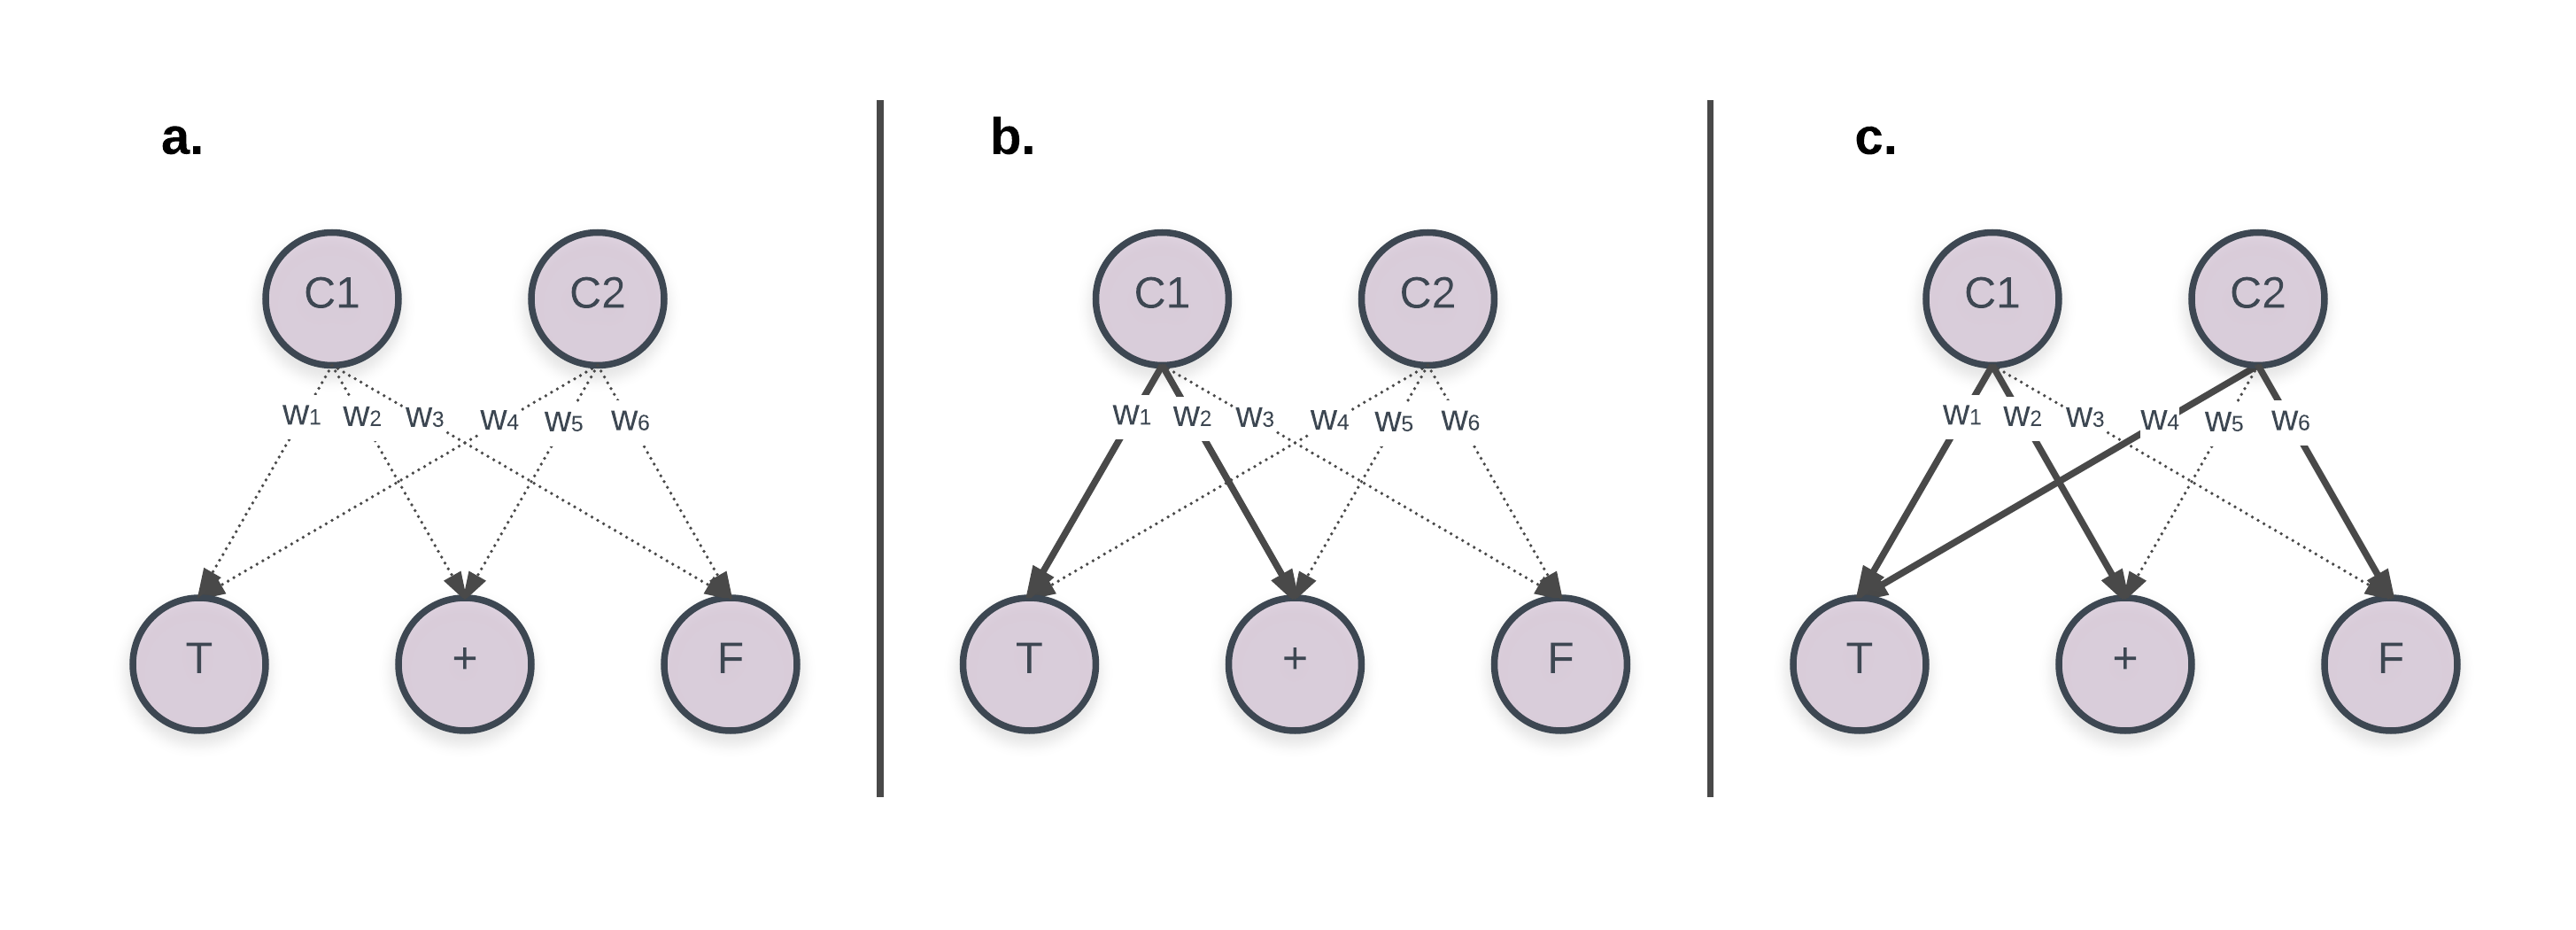
\includegraphics[width=\textwidth]{Figures/Fig5}
\caption{Latent causes C1 and C2 are assumed to generate certain environmental 
observations - namely, observations of the feature (F), the target (T), and 
reward ($+$); given an active cause, weight w gives the likelihood of making the 
associated observation. In general, OS is solved by associating the individual 
trial types with distinct latent causes. \bsf{(a)} Prior assumptions of the 
model are given by pre-existing connections between causes and events. \bsf{(b)} 
Upon experiencing a T$+$ trial, cause C1 is inferred by strengthening the 
appropriate weights. \bsf{(c)} L $\rightarrow$ T$-$ observations become linked 
with latent cause C2.}
\label{fig:latentCause}
\end{figure} 

It can be shown that this model can acquire the stimulus contingencies specific 
to trial types in OS. For example, if a reward ($+$) is consistently delivered 
whenever a target cue (T) sets off (i.e., a T$+$ trial), weights w$_{1}$ and w
$_{2}$ will be adjusted, thereby reflecting the knowledge that tone predicts 
reward (Figure 5a and 5b). This corresponds to the inference of latent cause 
C1, since the correlation of observations T and $+$ is causally attributed to 
C1 by virtue of the adjusted parameters.

It is relevant to consider what would happen if something in the environment 
changed. For example, if all of a sudden the animal received a feature cue (F) 
followed by the familiar T, but this time resulting in no reward (i.e., a F $
\rightarrow$ T$-$ trial, exactly as in NOS), the model should ideally detect 
this novelty, and update beliefs about cue relations appropriately. To account 
for this situation, \citeN{Courville2006} designed the model to make trial-by-
trial inferences as to whether parameters \textbf{w} have changed. As such, 
upon experiencing a F $\rightarrow$ T$-$ trial, the model would infer a likely 
change in parameters \textbf{w} due to the low value of the prior P(observation 
$\given$ \textbf{w}). This would result in a Bayesian update of the posterior, 
thereby revising beliefs about the structure of the world. More specifically, 
the model would learn event relations on F $\rightarrow$ T$-$ trials by 
strengthening weights w4 and w6 on the links between a previously irrelevant 
cause C2, and the appropriate events. This learning update is reflected in 
Figure 5 in the difference between parts b and c. Clearly, the model presented 
by \citeN{Courville2006} can handle occasion setting - inferring C1 or C2 
corresponds to an expectancy of a T$+$ or a L $\rightarrow$ T$-$ trial, 
respectively.

Despite this success, the model involves a number of disadvantages that are 
worth pointing out. Firstly, the model is only effective in learning to predict 
observations insofar as these are incorporated in its priors; clearly, this 
assumption becomes unfeasible in hyperdimensional, real-world situations 
composed of innumerable events (see \citeNP{Gershman2010a}). A further 
complication is the assumption of a finite parameter space \textbf{w} - the 
number of latent causes included is essentially stationary, and so any novelty 
in the environment must be modeled as a change in weights on existing causal 
links. This is a significant limitation, given that the model constrains the 
animal's experiences to a finite number of observations.

This problem is addressed in a variant of the generative model proposed by 
\citeN{Gershman2010b}. The authors present a normative Bayesian statistical 
framework that involves generative and inferential models designed to tackle 
conditioning phenomena such as renewal and latent inhibition. The model was 
inspired by a previously described TDRL algorithm that had additionally been 
designed to carry out state splitting \cite{Redish2007}. A crucial aspect of 
the \citeN{Gershman2010b} model is that it involves an infinite parameter space 
- given an observation, the model classifies it into a cluster of observations 
that corresponds to a common latent cause. In case the observation is not 
easily categorized into existing clusters, it is classified into its own 
separate cluster, thus corresponding to a novel latent cause. This procedure is 
formally known as the Dirichlet process, and has often been illustrated by a 
metaphor dubbed as the Chinese Restaurant process (see Box 1). Overall, this 
allows the model to account for the large number of distinct observations that 
animals encounter.

\begin{figure}[h]
\centering
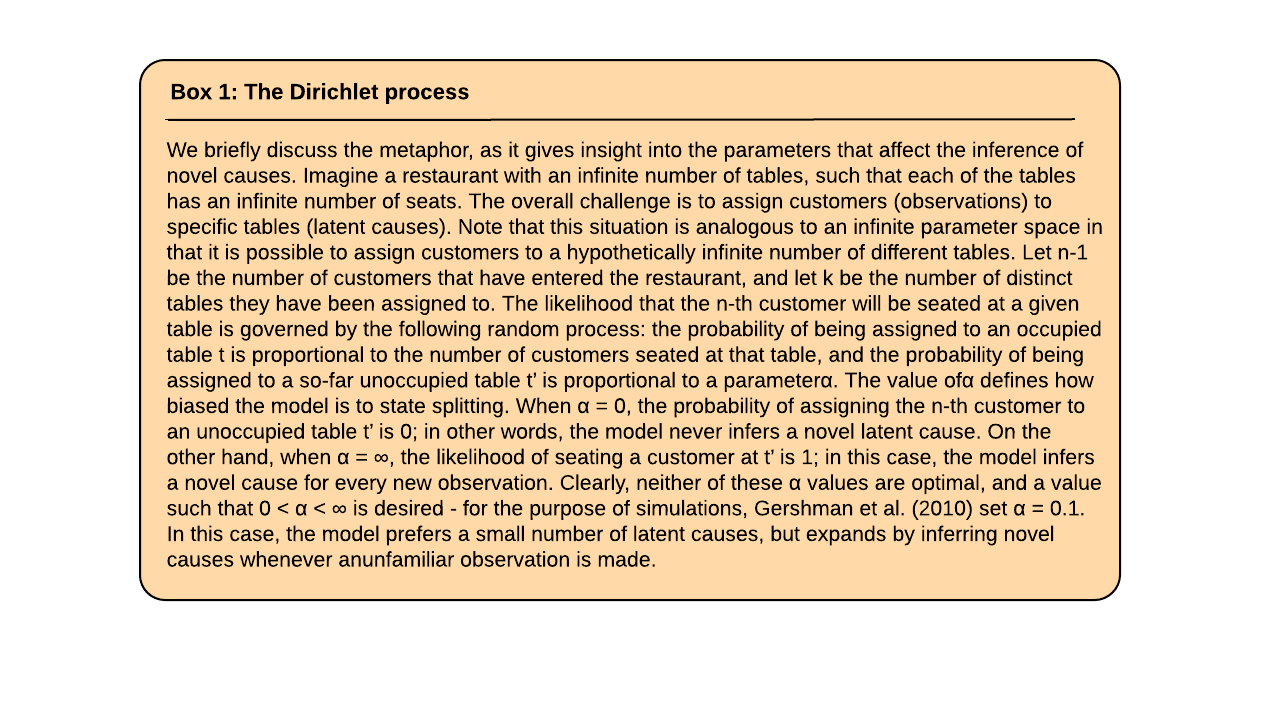
\includegraphics[width=\textwidth]{Figures/Box1}
\label{fig:dirichlet}
\end{figure}

\section*{Behavioral Predictions}

When a subject receives OS training (interspersed F $\rightarrow$ T and T 
trials), then according to a state-based account, F comes to control 
differential responding by prompting the agent to infer a novel state within 
which T comes to hold a different value. According to this view, the speed at 
which the discrimination is acquired depends on the degree to which the agent 
is prone to inferring novel states (e.g., within the latent cause theory, it is 
proportional to the parameter $\alpha$; see Box 1) From this new perspective on 
OS acquisition follow a number of behavioral predictions.

If the additional state that is required to solve OS were already inferred, the 
discrimination ought to be acquired more rapidly. This prediction can be tested 
by training animals in two consecutive OS regimes. In the first phase, animals 
are trained in an OS paradigm that consists of F $\rightarrow$ T and T trials 
(OS1). A state-based account posits that acquisition will involve using F to 
toggle a unique state within which T acquires a new meaning. This can be tested 
by commencing a second OS training schedule that involves F $\rightarrow$ T' 
and T' (OS2). In this second phase, F is already trained to toggle a unique 
state. As such, acquisition of OS2 should occur more rapidly than acquisition 
of OS1. 

A related prediction is that acquisition ought to proceed more rapidly if the 
rewarded state is made more distinct from the unrewarded state. One possibility 
would be to make F more salient. However, increasing the salience of F relative 
to that of T is known to promote conditioned inhibition, a form of learning 
that is distinct from OS. Given that acquisition of OS is highly parameter-
dependent \cite{Holland1992}, it is not trivial to determine which manipulation 
would make the ``F'' state more distinct from the ``no F'' state whilst 
preserving all the parameters that normally favor acquisition of OS. However, 
one interesting option might be to make F long. Prolonging dwell time in the 
``F'' state might make it more different from the ``no F'' state, thus 
increasing the rate of OS acquisition. This manipulation simulates the 
effective presence of a distinct context (e.g., lighting of the conditioning 
chamber that persists), thereby making the task similar to contextual OS, which 
is generally acquired faster than discrete-cue OS (cite!!!). 

A conceptually similar manipulation is to alter the rate of OS acquisition by 
making the ``F'' state perceptually similar to the ``no F'' state. This would 
render the inference of a novel state more difficult, thereby slowing the rate 
of acquisition. Experimentally, this can be achieved by signaling the ``F'' and 
``no F'' states with background lights of similar light intensities. 
Interestingly, \citeN{Gershman2013} successfully tested this general idea by 
taking advantage of the renewal effect. Renewal comprises three distinct phases; 
first, a CS-US contingency is acquired in a conditioning context. Next, the CS 
undergoes an extinction phase in which conditioned responding is reduced by 
repeatedly presenting the CS in the absence of the US (CS-noUS). In a crucial 
test, the animal is moved outside the extinction context, and expresses 
resurgence of responding (i.e., renewal) when it next encounters the CS 
\cite{Bouton2004}. It is thought that the extinction phase produces a novel CS-
US contingency whose retrieval depends on contextual disambiguation. In the 
language of a state-based account, the animal infers a new state in the 
extinction context, which explains why extinction learning does not generalize 
to other context. \citeN{Gershman2013} tested this idea by presenting a mix of 
CS-US and CS-noUS trials in the extinction phase, such that the proportion of 
CS-noUS trials gradually increased later in the session. This was hypothesized 
to make the extinction context more similar to the conditioning context, thereby 
preventing the inference of a novel state. Consistent with this idea, the 
renewal effect was not observed when the animals were tested outside the 
extinction context.  

\section*{Neural Predictions}

We have argued above that ambiguity resolution requires a segmentation of
experience into distinct states, wherein otherwise ambiguous target stimuli 
acquire a clear meaning. The problem of resolving ambiguities therefore becomes 
a problem of acquiring an appropriate state space. The latent cause theory is a 
plausible algorithmic answer to this conundrum. In the present section, we 
briefly discuss two brain regions that are well-positioned to implement such a 
process: namely the hippocampus (HC), and the orbitofrontal cortex (OFC) (see 
\citeNP{Wikenheiser2016} for a detailed review on state encoding in these 
regions). We conclude by suggesting specific neurophysiological manipulations 
that will shed light on the flow of information across these regions in a task 
like NOS. 

{\bf Evidence for State Encoding in HC and OFC} 

The concept of state space is related to Tolman's notion of a cognitive map 
\cite{Tolman1948}. Within this framework, subjects infer the variables that are 
relevant for current behavioral demands, and update an internal relational map 
of their environment that is recruited in order to drive adaptive behavior. In 
a similar vein, state spaces enable behavioral flexibility by segmenting 
experience into discrete chunks whose contents can often be contradictory 
(e.g., respond to T in ``no F'' state, withhold response in ``F'' state, as in 
NOS). The benefits of maintaining a state space are equivalent to those 
provided by a map - each reduces uncertainty about the environment. 

Hippocampal place cells selectively fire in localized regions of space that 
tile the animal's environment \cite{OKeefe1971,OKeefe1978}; for this reason, 
the hippocampus is the brain region most commonly thought of as storing a 
Tolmanian cognitive map. There are a number of ways to conceptualize state 
representations in the hippocampus, and these depend on different levels of 
granularity. 

At the single cell level, the spatial field a `place cell' responds to can be 
thought of as representing a discrete state in a spatial map. Interestingly, a 
recent article by \citeN{Stachenfeld2017} recasts this long-standing idea by 
proposing that single place cells encode expectations of a fixed future state 
given the current state; this frames the hippocampus as a predictive spatial 
map. In any case, the entire population of responsive place cells forms a 
macrostate that represents the animal's current context (e.g., conditioning 
chamber). The importance of this emerges when the animal is placed in a novel 
context. Place cells undergo a transition to a novel state (traditionally 
referred to as a `remapping') in which they acquire tuning that is often 
completely unrelated to that in the former context 
\cite{Muller1987,Muller1996}. Not surprisingly, performance in a variety of 
tasks that depend on successful retrieval of context-dependent information is 
typically impaired in animals with a damaged hippocampus 
\cite{Honey1993,Holt1999,Gilbert2001,Corcoran2004,Maren2013,Xu2016}. 

A somewhat different picture of state encoding emerges at the level of 
sequential place cell activity. As the animal moves through its environment, 
sequences of place cell firing track a specific behavioral trajectory. 
Crucially, these sequences also occur at faster time-scales, and sometimes 
extend beyond the animal's immediate location. \citeN{Johnson2007} demonstrated 
that this tends to occur as the animal prospectively samples options before 
making a decision (often dubbed as `vicarious trial and error'; see 
\citeNP{Tolman1939,Redish2016}). At the choice point, hippocampal sequences 
extended along potential paths to reward before the animal set out. In other 
words, the sequences reflect internal simulations of alternative trajectories 
towards reward. Each can be thought of as a distinct state whose value depends 
on the animal's belief as to which trajectory is currently rewarded. Crucially, 
the contents of hippocampal sequences are not exclusively spatial. A number of 
studies have demonstrated that delay periods requiring maintenance of past 
information to inform a future response (e.g., delayed T-maze alternation and 
match-to-sample tasks) are characterized by hippocampal sequences that are 
predictive of subsequent behavior 
\cite{Pastalkova2008,MacDonald2011,MacDonald2013}.

Apart from the hippocampus, a number of areas in the prefrontal region have 
been implicated in state learning. Consistent with its general role in 
cognitive control 
\cite{Botvinick2001,Liston2006,Casey2005,Haddon2006,Haddon2007,Braver2012}, the 
prefrontal cortex (PFC) has been framed as an executive controller that uses 
task-dependent event-outcome relations to mediate processing in downstream 
regions \cite{Miller2000}. For instance, medial PFC undergoes population-level 
shifts in network dynamics during changes in task structure 
\cite{Durstewitz2010,Karlsson2012}, which are thought to reflect a formation of 
discrete states that support disparate rules. 

Furthermore, a great deal of evidence suggests that orbitofrontal cortex (OFC) 
plays an important role in state space acquisition. First, a well-functioning 
OFC is necessary to maintain behavioral flexibility in the face of a 
dynamically changing environment \cite{Bechara1994}. For instance, animals with 
OFC lesions show deficits in reversal learning 
\cite{Schoenbaum2003a,Delameter2007}, which requires the inference of novel task 
contingencies, and an update of current behavioral strategy. Second, OFC 
represents the current value of relevant events. Its neurons track stimuli that 
are predictive of a specific outcome, and thereby abstract beyond value 
encoding that is linked to a specific stimulus 
\cite{Schoenbaum1998,Baxter2000,Schoenbaum2003b}. Furthermore, OFC neurons have 
the capacity to decompose an event into its components (e.g., informativeness, 
value, etc.), and represent these via orthogonal codes \cite{Blanchard2015}. 
These seemingly disparate roles - i.e., behavioral flexibility and value 
encoding - are consistent with a recent theory of OFC function. 
\citeN{Wilson2014} suggest that unexpected changes in task contingencies (as 
in serial reversal learning) are handled by inferring OFC states whose contents 
store the values of relevant events. To test this hypothesis, the authors 
modeled OFC lesions as an inability to maintain more than one state at a time. 
Amazingly, this simple assumption was sufficient to account for a large body of 
research detailing the effects of OFC lesions on behavior in a number of 
related tasks (e.g., reversal learning, extinction, devaluation, delayed 
alternation, etc.). Crucially, OFC states are thought to be more abstract, 
encoding task variables that are not explicitly observed, and must therefore be 
inferred \cite{Bradfield2015,Stalnaker2015}.

Indeed, HC and OFC likely cooperate by contributing unique components to a more 
holistic state space representation \cite{Wikenheiser2016}. In a T-maze 
alternation task, distinct OFC neurons selectively fire at each of the reward 
sites \cite{Steiner2012}. Surprisingly, during periods of `vicarious trial and 
error' (as described above), these representations of far-away reward become 
active. It is plausible that this corresponds to an assignment of value to the 
behavioral trajectories simulated in the hippocampus, resulting in a complex, 
multidimensional state space that allows exploration of spatial trajectories in 
the service of obtaining reward. The anatomical connectivity between OFC and HC 
certainly supports this hypothesis: while projections from OFC to HC are 
indirect \cite{Prasad2013}, those from HC to OFC are direct 
\cite{Jay1991,Barbas1995}. This suggests the interesting possibility that 
simulated `lookaheads' in HC cue the OFC, which imbues the simulated 
trajectories with biological meaning. Overall, our working hypothesis suggests 
that HC and OFC coordinate in order to store a state space that is drawn upon 
to enable adaptive behavior. Given that OFC and HC projections converge on the 
nucleus accumbens (NAcc) \cite{Mogenson1980}, we propose that state information 
is passed down to this region in order to promote context-appropriate behavior. 
NAcc is a suitable candidate for this downstream processing, given its role in 
invigorating reward-related responding based on interactions with frontal and 
temporal regions \cite{Floresco2015}. Furthermore, a number of studies have 
already demonstrated that activity between HC/OFC and NAcc is tightly 
coordinated \cite{Cooch2015,VanderMeer2011}. Next, we explore the putative 
roles of these regions in ambiguity resolution.

{\bf Neurobiology of Ambiguity Resolution}

Apart from discussing the roles of HC and OFC in state encoding, the previous 
section already implies their involvement in ambiguity resolution. Both of 
these regions are crucial in a number of ambiguity resolution tasks listed in 
Figure 1 (e.g., T-maze alternation, delayed match-to-sample, serial reversal 
learning, etc.). As such, it is unsurprising that HC and OFC have been 
implicated in OS.  

Only a handful of studies have investigated the role of prefrontal regions in 
OS. For instance, simultaneously disrupting activity in OFC and NAcc leads to 
protracted acquisition of NOS \cite{Meyer2016}. A related study showed that 
pretraining lesions of the mPFC prelimbic region retard acquisition of NOS, 
consistent with this region's role in acquiring behavioral strategies 
(\citeNP{MacLeod2010}; also see \citeNP{Meyer2014}). These results suggest 
that OFC and mPFC play a role in the acquisition of NOS.

Although there has been more research into the role of HC in OS, results have 
been mixed. While aspiration lesions prevented acquisition of POS 
\cite{Ross1984}, ibotenic acid lesions had no effect \cite{Jarrard1990}. Both 
of these results were replicated by \citeN{Jarrard1991}, who also observed that 
aspiration lesions produced greater extra-hippocampal damage than ibotenic acid 
lesions. The authors concluded that the deficit in POS resulted from damage to 
structures outside the hippocampus. A number of later studies corroborated this 
conclusion \cite{Moreira2003,Holland1999}. Interestingly, \citeN{Holland1999} 
further found that neurotoxic hippocampal lesions caused a marked deficit in 
acquiring NOS. These results point to an interesting asymmetry behind HC's 
involvement in acquiring POS as opposed to NOS. It is plausible that a deeper 
investigation of this phenomenon may help us understand the neural basis of the 
feature-positive effect.

While these studies suggest that OFC and HC are involved in the acquisition of 
OS, the existing literature leaves a great deal to be desired. To our 
knowledge, no one has investigated whether OFC, HC, and NAcc are necessary for 
the performance of OS. This question could be probed by reversibly inactivating 
each region at peak performance using chemogenetic tools such as DREADDs. 
Furthermore, the nature of information flow across these regions remains 
largely unknown. To this end, reversible disconnections between all pairs of 
regions would help establish whether communication between them is necessary 
for acquisition (disconnect throughout training) or performance (disconnect at 
peak responding). After establishing the macro-scale interactions that support 
OS, a more fine-grained investigation would need to be conducted to reveal the 
neural interactions that are necessary for correct responding within a single 
trial. On any given trial, the correct state must be toggled based on the 
presence or absence of the feature (presumably, this occurs in HC and OFC), and 
this information must ultimately reach NAcc in order to facilitate responding 
once the target cue comes on. It is unclear, however, whether this information 
transfer occurs all throughout the interstimulus interval, if it is confined to 
the period of the feature cue, or to the period of the target. These 
interesting possibilities can be parsed out by optogenetically inactivating 
each region during periods of interest (i.e., interstimulus interval, target 
presentation). Lastly, large-scale electrophysiological recordings would need 
to be conducted in order to identify the nature of information being coded. It 
is of particular interest whether network activity could be successfully 
decoded to predict the animal's response on any given trial. 

In fact, the first steps in this direction have already been made by 
\citeN{Shobe2017}, who recorded from a population of OFC neurons while head 
restrained mice performed a NOS task. The proportion of OFC neurons whose 
firing rates discriminated between rewarded and unrewarded instances of the 
target correlated with performance on the task. More importantly, however, the 
authors discovered that during the interval preceding target presentation, OFC 
network activity was significantly different on rewarded versus unrewarded 
trials. Furthermore, this network state was identical irrespective of 
performance to the upcoming target. Even though OFC state does not predict 
trial performance, it is possible that it alters activity in a downstream 
region (e.g., NAcc), where upcoming performance could be decoded. This again 
begs the question whether OFC needs to be online during the interstimulus 
interval, underscoring the importance of the manipulations we propose above. 

\bibliography{os_review}{}

\end{document}
